\documentclass[8pt, twocolumn]{article}
\usepackage{amsmath}
\usepackage{graphicx}
\usepackage[margin=0.75in]{geometry}

\author{Jaime Guerrero}
\title{Parallelization of Karatsuba's Algorithm using Cilk}
\date{\today}

\begin{document}

\maketitle

\section{Overview}
\textbf{Put some more about Cilk programming}
I provide a implementation of Karatsuba's multiplication algorithm that has
been parallelized with the Cilk extensions to C.  By taking a correct,
sequential version of the program, impressive speedups are possible with
minimal programmer effort.

\section{Background}
The sequential C implementation of Karatsuba's algorithm is from the capstone
project for Paul Purdom's \textit{Algorithm Design and Analysis} class taken in
Spring 2014.  The goals of this project are twofold: the first is to have the
fastest implementation possible when compared to other students in the class.
The second goal is to carefully analyze an algorithm, given the constraints of
a machine's architecture.  With the help of Tim Zakian and Spenser Bauman, the
sequential version presented here was the fastest of that semester.

\section{The Setup}
The GMP library is used to generate random numbers which are then multiplied
by both the implementation of Karatsuba's algorithm, as well as the built-in
GMP multiplication routine.  Because of GMP's highly optimized multiplication
routines, I was able to compare Karatsuba's algorithm for both speed and
correctness.

Karatsuba's multiplication algorithm takes a divide-and-conquer approach to
the classic problem of multiplying numbers.  Where the traditional, ``naive''
algorithm is $O(n^2)$ in the number of bits being multiplied, Karatsuba's
algorithm is $O(n^{\log_2 3})$ in the number of bits.  This speedup is gained
through a reduction in the number of multiplications that must be done in
exchange for a few more additions.

In the vein of most divide-and-conquer algorithms, Karatsuba is amenable to
parallelization.  Rather than waiting for sequential processes to work upon one
half of the data at a time, both haves can be worked upon in parallel, with
their answers combined toward the end of the computation.

The programming model provided by Cilk was a natural choice for this project.
Cilk's fork-join approach to parallelism makes it easy to know where to place
calls to \texttt{cilk\_spawn} and \texttt{cilk\_sync}. Furthermore, Cilk's
serial elision property ensures that changes to that my program retains its
intended semantics, but simply runs faster.

\section{Benchmarks}

\begin{figure}[t]
    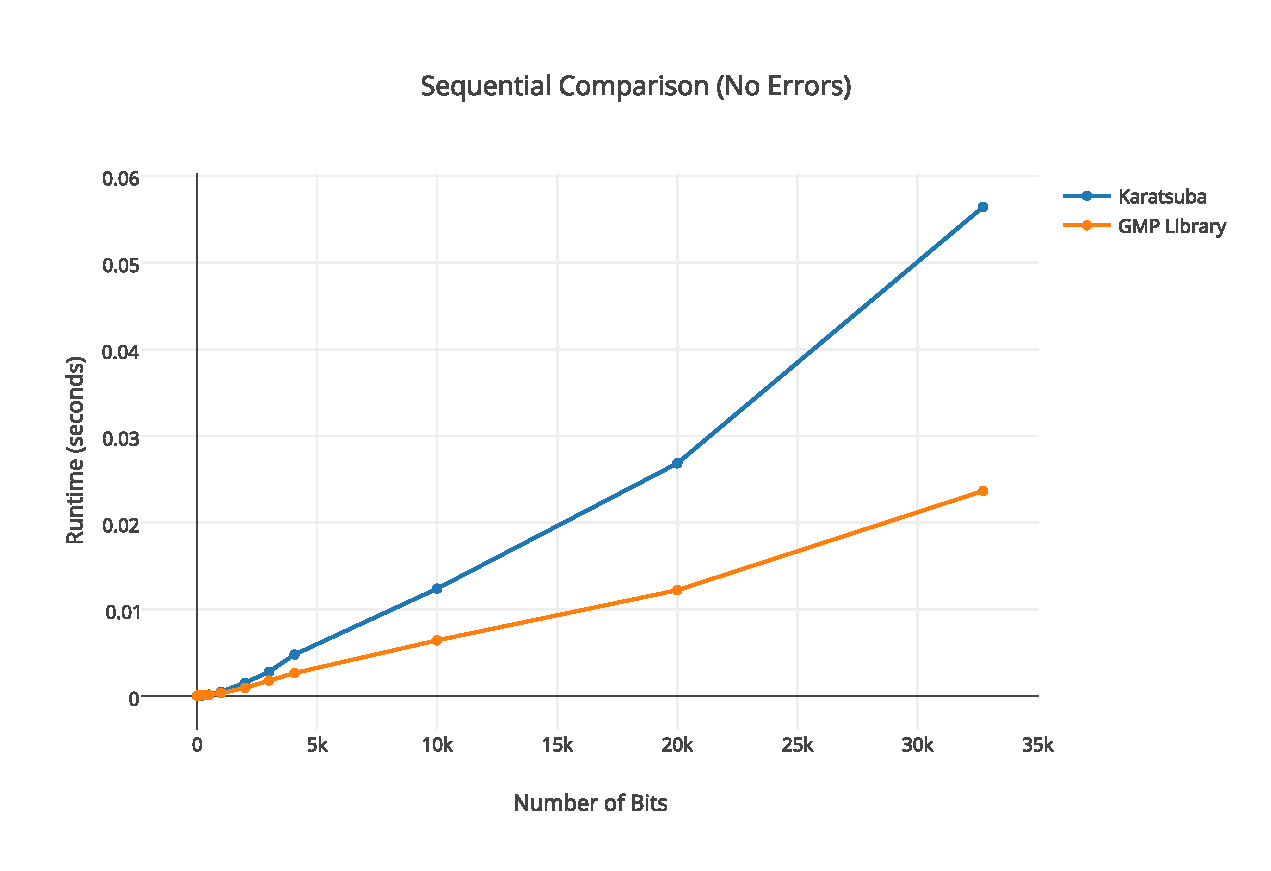
\includegraphics[scale=0.4]{sequential-error-free}
    \caption{Runtimes of sequential Karatsuba and GMP, wherein all Karatsuba answers
    are correct.}
    \label{fig:sequential-correct}
\end{figure}

All tests were run on ``Wolverine'', an 8-core, 64-bit machine running Red Hat
Linux version 2.6.32 with 16 GB of RAM.  Several optimizations were applied to
the sequential version of the code.  The most interesting are detailed below:
\begin{enumerate}
    \item \texttt{-march=native} switch: Allows for highly specialized compilation
          that is tuned to the machine's architecture.
    \item \texttt{-fomit-frame-pointer} switch: Provides an extra register when the
           frame-pointer does not need to be kept around.
    \item \texttt{-fdelete-null-pointer-checks} switch:  Do not check for null
          pointers.
    \item \texttt{-fif-conversion2} switch: Per the online GCC manual, ``Transforms
          conditional jumps into branch-less equivalents''.
    \item \texttt{((flatten))} pragma: inline as much of a function's body as
          possible.
    \item \texttt{((nothrow))} pragma: note that a function will not throw an
          exception.
\end{enumerate}

Regardless of the number of optimizations enabled, poorly structured code will
still run slowly.  To that end, the code was written in a way that would
minimize memory allocation/deallocation, as well as grouping together repeated
function calls.

The main program driver runs both the GMP multiplication routine and Karatsuba's
algorithm 100 times; the running time of both (in seconds) is charted below.
When this program was originally written, it was tested on numbers not exceeding
32736 bits, and all answers were correct.  Figure \ref{fig:sequential-correct} shows the
benchmarks for the very first implementation from Purdom's class.

For the sake of fully exploring the implementation, I experimented with inputs
of varying sizes.  At around two-hundred thousand bits, the sequential Karatsuba
begins to produce wrong answers, while the parallel version produces wrong
answers at four million bits.  To that end, the only measurements presented here
were those that were correct.  The cause for these wrong answers is unknown.  It
was originally believed to be a matter of freeing all allocated memory; this
remedied all incorrect answers in the parallel version for ``small'' inputs,
though did not scale as expected.

Since the 8 and 16 workers versions are so similar in their runtimes, I have
only included the 8 worker for the sake of space.

\begin{figure}[t]
    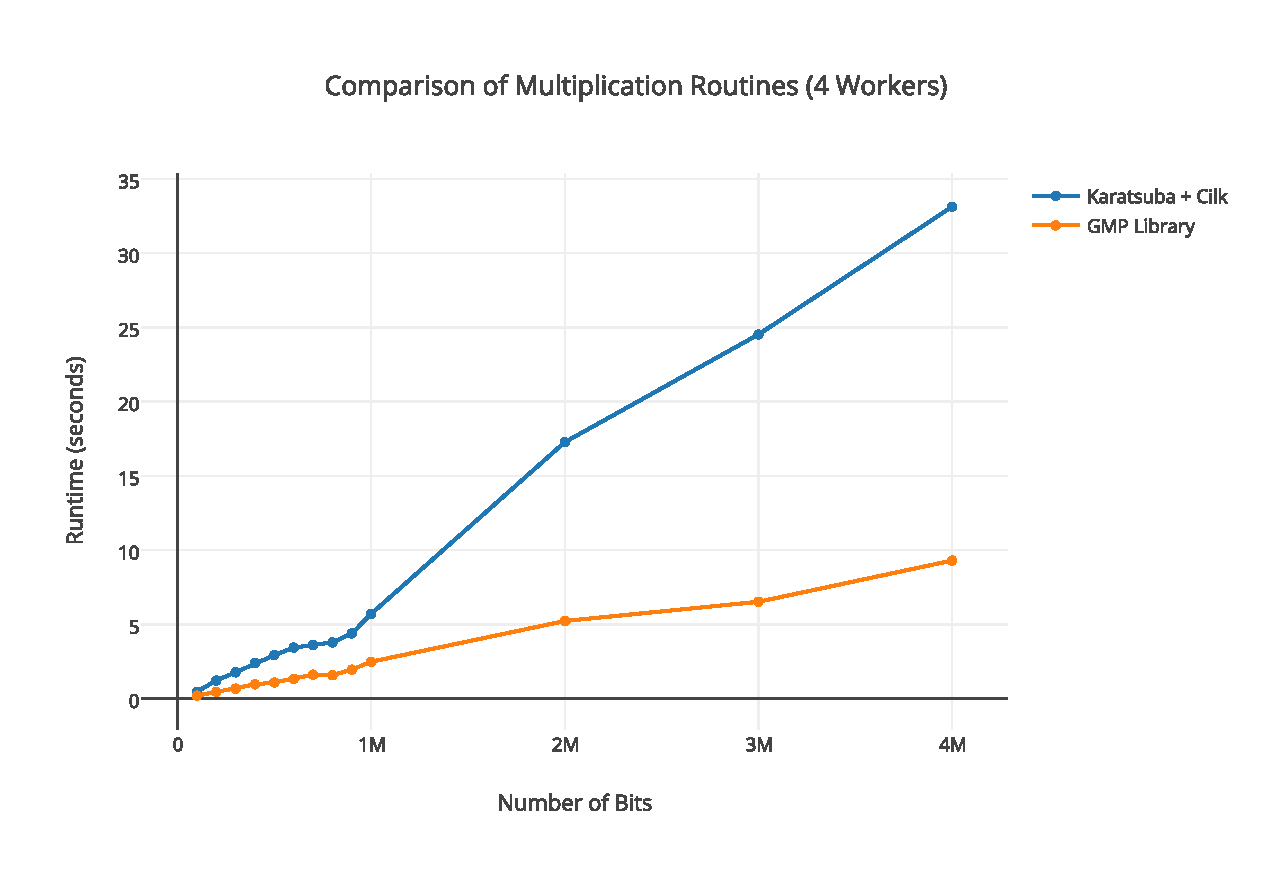
\includegraphics[scale=0.4]{4-workers}
    \caption{Comparison of GMP with 4 Cilk workers.}
    \label{fig:4-workers}
\end{figure}

\begin{figure}[t]
    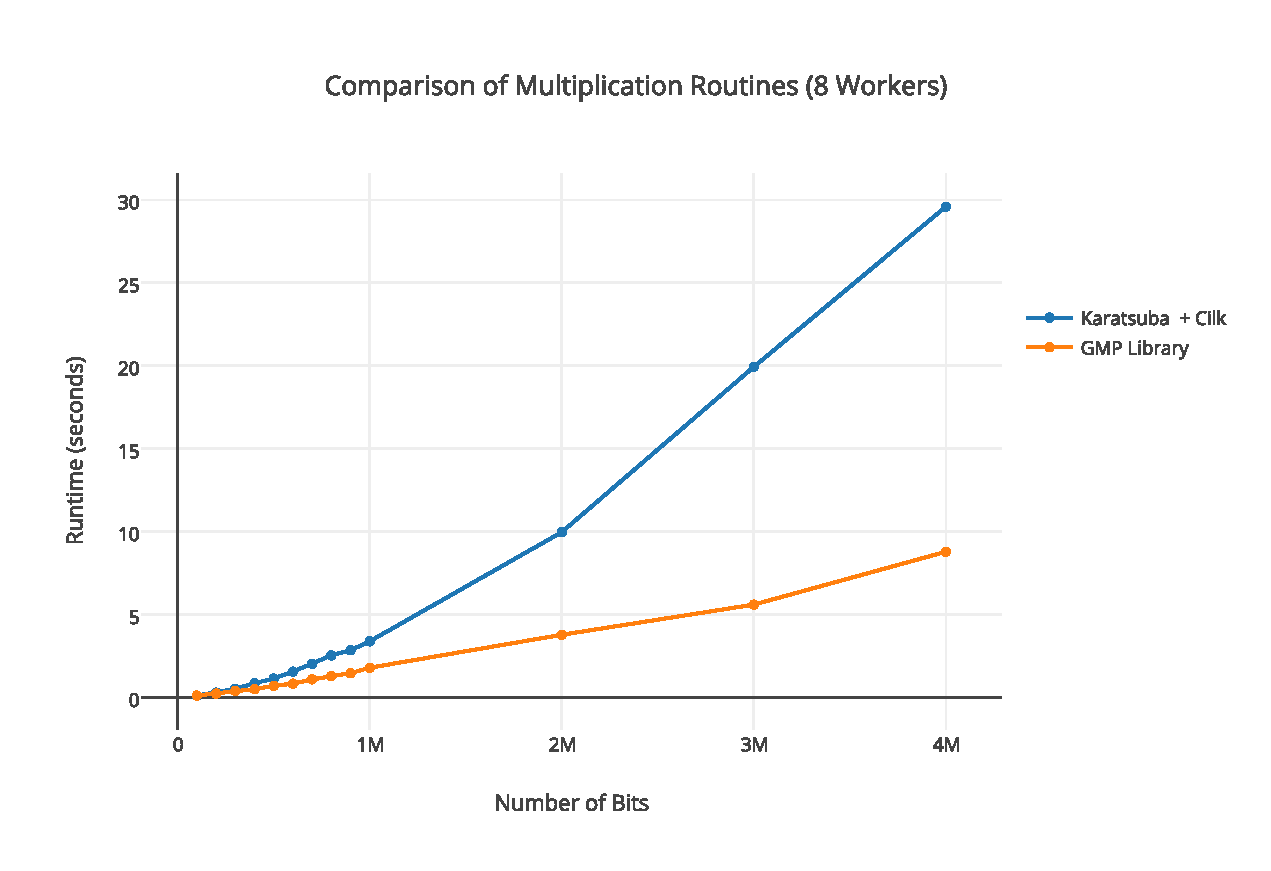
\includegraphics[scale=0.4]{8-workers}
    \caption{Comparison of GMP with 8 Cilk workers.}
    \label{fig:8-workers}
\end{figure}

\begin{figure}[t]
    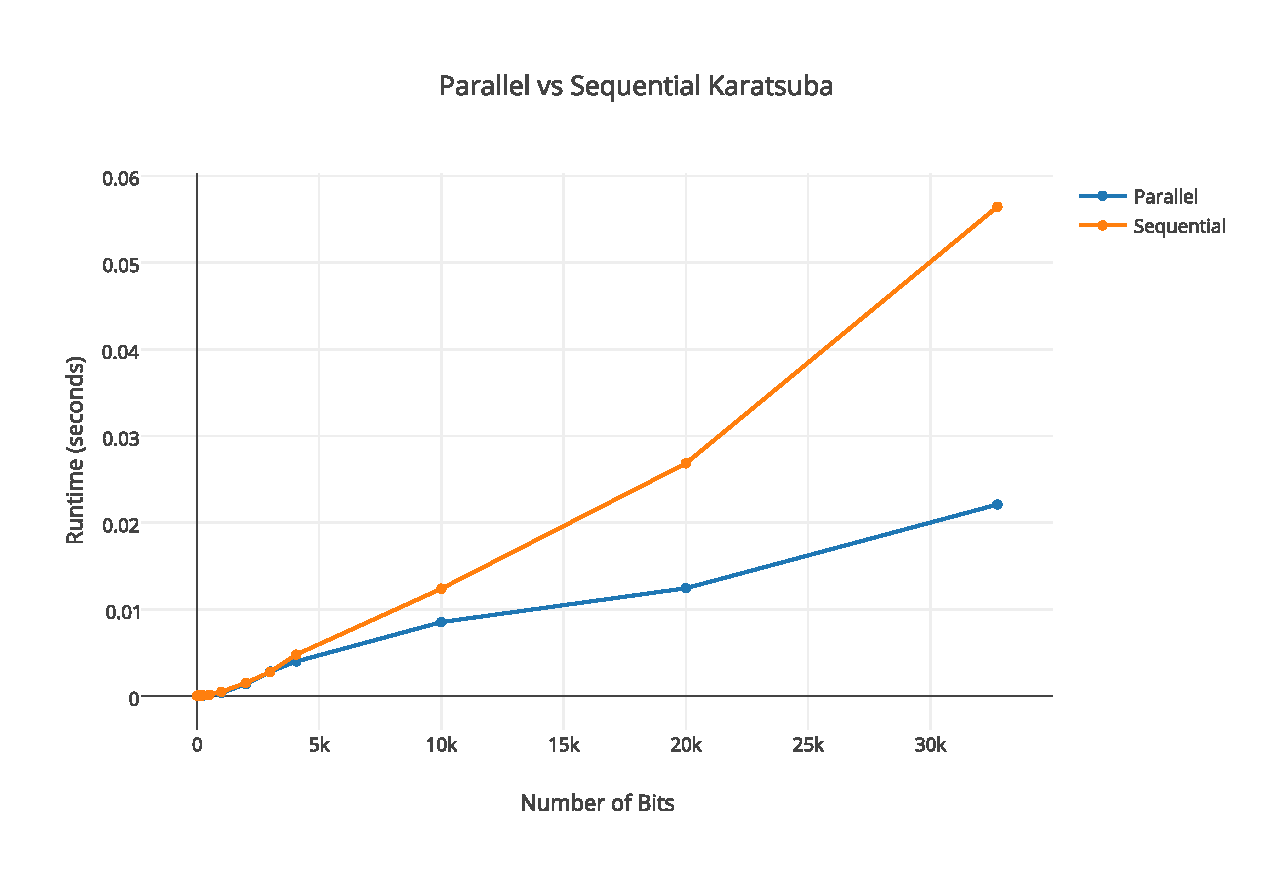
\includegraphics[scale=0.4]{parallel-vs-sequential}
    \caption{Parallel performance in comparison to sequential implementation.}
    \label{fig:parallel-vs-sequential}
\end{figure}


Figure \ref{fig:parallel-vs-sequential} demonstrates that Cilk's speedup with
four workers is appreciable when compared to the sequential implementation.
Both Figure \ref{fig:4-workers} and Figure \ref{fig:8-workers} show that the
parallel algorithm is competitive with the GMP routine up until around one
million digits.  The dropoff of Karatsuba is most pronounced in the 4-worker
version.  However, the overall performance of the parallel version is better
than the sequential implementation.

GMP has the benefit of hundreds of developer hours and more sophisticated
multiplication routines, and it is clearly the superior choice when speed is the
main requirement.  However, the Cilk library provides a solid performance
improvement and a low barrier to entry that makes it an attractive tool for the
average programmer.

\section{Acknowledgements}
Thanks to Spenser Bauman and Tim Zakian for their help with the sequential
version.

%\section{Full Algorithm}
%The Karatsuba multiplication algorithm as outlined by Purdom and Brown.
%
%Input: the $2n$-bit number $U = U_1 2^n + U_2$ where $0 \leq U_1 < 2^n$ and $0
%\leq U_2 < 2^n$, and the $2n$-bit number $V=V_1 2^n + V_2$ where $0 \leq V_n
%< V^n$.  Output: The product $UV$ represented by $UV = W_1 2^{3n} + W_2 W^{2n} + W_3 2^n + W_4$.
%
%\begin{itemize}
%    \item Set $T_1       := U_1 + U_2$
%    \item Set $T_2       := V_1 + V_2$
%    \item Set $W_3       := T_1 T_2$
%    \item Set $W_2       := U_1 V_1$
%    \item Set $W_4       := U_2 V_2$
%    \item Set $TempDiff  := W_3 - W_2$
%    \item Set $TotalDiff := TempDiff - W_4$
%    \item Set $Carry     := \lfloor W_4 / 2^n \rfloor$
%    \item $W_4            = W_4 \mod 2^n$
%    \item Set $\hat{W_3}  = TotalDiff + Carry$
%    \item Set $\bar{C}    = \lfloor \hat{W_3} / 2^n \rfloor$
%    \item $W_3            = \hat{W_3} \mod 2^n$
%    \item Set $\hat{W_2} := W_2 + \bar{C}$
%    \item $W_1            = \lfloor \hat{W_2} / 2^n \rfloor$
%    \item $W_2            = \hat{W_2} \mod 2^n$
%\end{itemize}


\end{document}
